\subsection{Synthetic Data}

The first experiment uses the 500 data points (Figure \ref{fig:experiment1_data}) generated from a three state EDHMM. The duration distributions were Poisson with rates $\lambda_1 = 5$, $\lambda_2 = 15$, $\lambda_3 = 20$; each observation distribution was Gaussian with means of $\mu_1 = -3$, $\mu_2 = 0$, and $\mu_3 = 3$, each with a variance of 1. The transition distributions $A$ were set to
\begin{equation*}
\begin{bmatrix}
    0 & 0.3 & 0.7 \\ 0.6 & 0 & 0.4 \\ 0.3 & 0.7 & 0
\end{bmatrix}.  
\end{equation*}

\begin{figure}
    \subfloat[][]{
        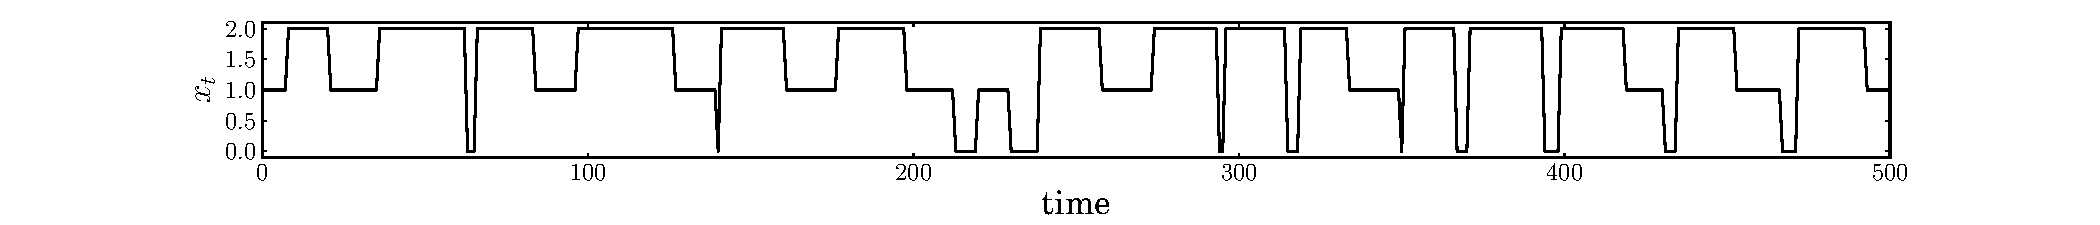
\includegraphics[width=0.5\textwidth]{../pic/experiment_2_X.pdf}
        \label{fig:exp_1_state}
    } \\
    \subfloat[][]{
        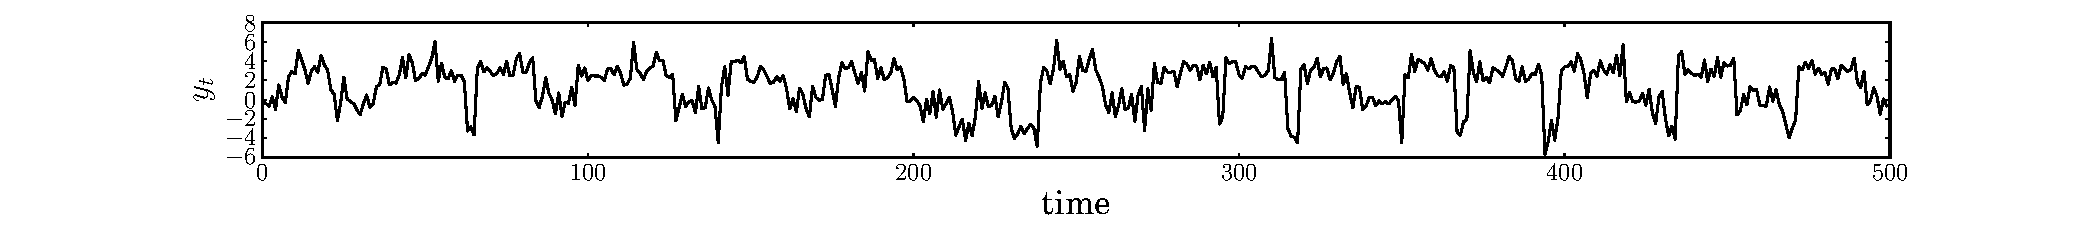
\includegraphics[width=0.5\textwidth]{../pic/experiment_2_Y.pdf}
        \label{fig:exp_1_data}
    }
    \caption{Example a) state and b) observation sequence generated by the explicit duration HMM. Here $K$ = 3; $p(y_t|x_t=j) = \mathrm{N}(\mu_j, 1)$ with $\mu_1 = -3$, $\mu_2 = 0$, and $\mu_3 = 3$; and $p(d_t|x_t=j) = \mathrm{Poisson}(\lambda_j)$ with $\lambda_1 = 5$, $\lambda_2 = 15$, and $\lambda_3 = 20$.}
    \label{fig:experiment1_data}
\end{figure}

Broad, uninformative priors were chosen for the parameters of the duration and observation distributions. The observation distribution parameters were given a normal-inverse-Wishart (N-IW) prior with parameters $\nu_0 = 2$, $\Lambda_0 = 1$, $\kappa=0.1$ and $\mu_0 = 0$. The rate parameters for all states were given $\mathrm{Gamma}(1, 10^{5})$ priors. 

One thousand samples were collected from the EDHMM beam sampler after a burn-in of 500 samples. The learned posterior distribution of the state duration parameters and means of the observation distributions are shown in Figure \ref{fig:experiment1_results}.  The EDHMM achieves high accuracy in the estimated posterior distribution of the observation means, despite the overlap in observation distributions. The rate parameter distributions are reasonably estimated given the small number of observed segments. Figure \ref{fig:allowed} shows the mean number of transitions visited per time point over each iteration of the sampler. 

\begin{figure}
    \subfloat[][]{
        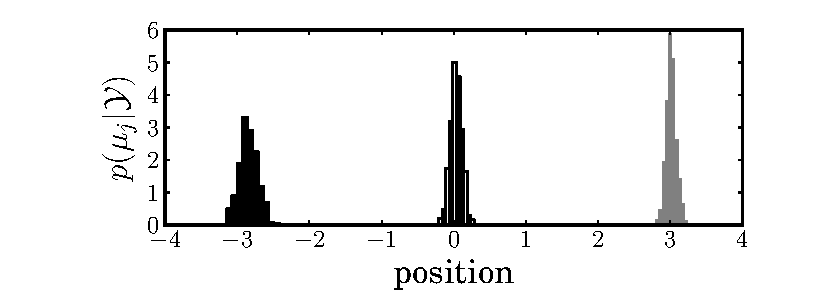
\includegraphics[width=0.25\textwidth]{../pic/posterior_means.pdf}
        \label{fig:posterior_means}
    } 
    \subfloat[][]{
        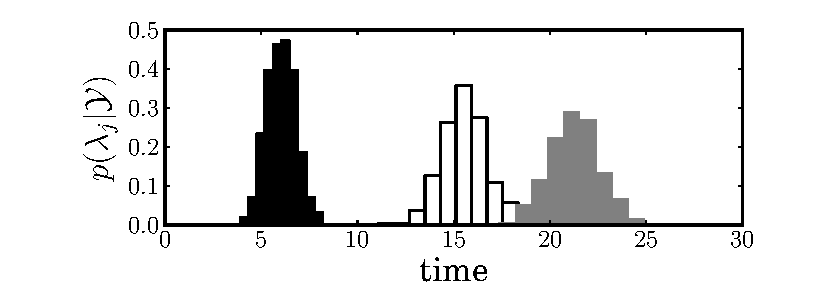
\includegraphics[width=0.25\textwidth]{../pic/posterior_rates.pdf}
        \label{fig:posterior_rates}
    }
    \caption{Samples from the posterior distributions of a) the observation distribution means and b) the duration distribution rate parameters for the data shown in Figure \ref{fig:experiment1_data}.}
    \label{fig:experiment1_results}
\end{figure}

\begin{figure}
    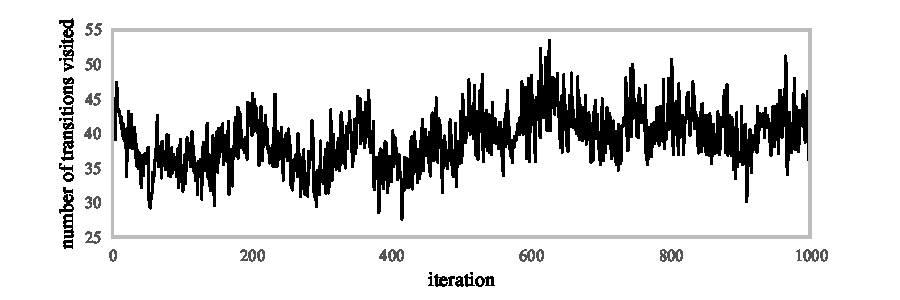
\includegraphics[width=0.45\textwidth]{../pic/number_transitions_visited.pdf}

\caption{Mean number of transitions considered per time point by the beam sampler for 1000 post-burn-in sweeps on data from Figure \ref{fig:experiment1_results}. Consider this in comparison to the $(KT)^2 = O(10^6)$ per time point transitions that would need to be considered by standard forward backward without truncation, a surely-safe, truncation-free, but computationally impractical alternative.}
\label{fig:allowed}
\end{figure}

A second experiment was performed to demonstrate the ability of the EDHMM to distinguish between states having differing duration distributions but the same observation distribution. The same model and sampling procedure was used as above except here $\mu_1 = 0$, $\mu_2 = 0$, and $\mu_3 = 3$.
Figure~\ref{fig:experiment2_results} shows that the sampler clearly separates the high state associated with $\mu_3$ from the other states and clearly 
%identifies the fact that there are 
reveals the presence of
two  low states with differing duration distributions. Figure~\ref{fig:exp_2_state} shows posterior samples that indicate that the model is mixing over ambiguities about states $0$ and $1$ as it should. %As shown in Figure \ref{fig:experiment2_results}, when the state transitions to and from the long-high state to the short-low state (e.g. $t\approx 100$ and $t\approx 180$) the transitions are captured well. When the system transitions between the two low states the segmentation is less accurate, due to the inherent lack of identifiability during these periods. Instead, the space of valid state sequences is explored, each sequence obeying the duration distribution.

%Despite the loss of identifiability in the state sequence, the sampler is still able to capture reasonable estimates for the parameters of the observation and duration distributions.

\begin{figure}
    \subfloat[][]{
        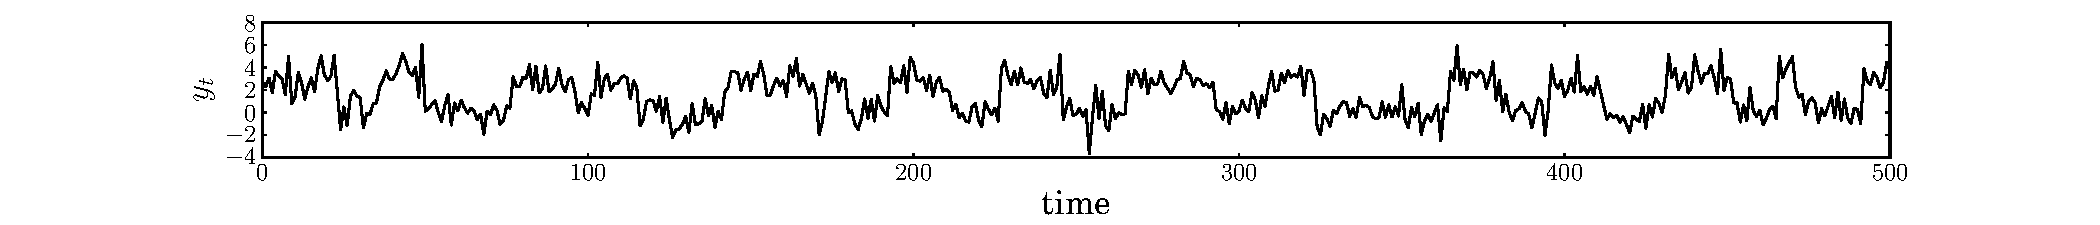
\includegraphics[width=0.5\textwidth]{../pic/experiment_3_Y.pdf}
        \label{fig:exp_2_data}
    } \\
    \subfloat[][]{
        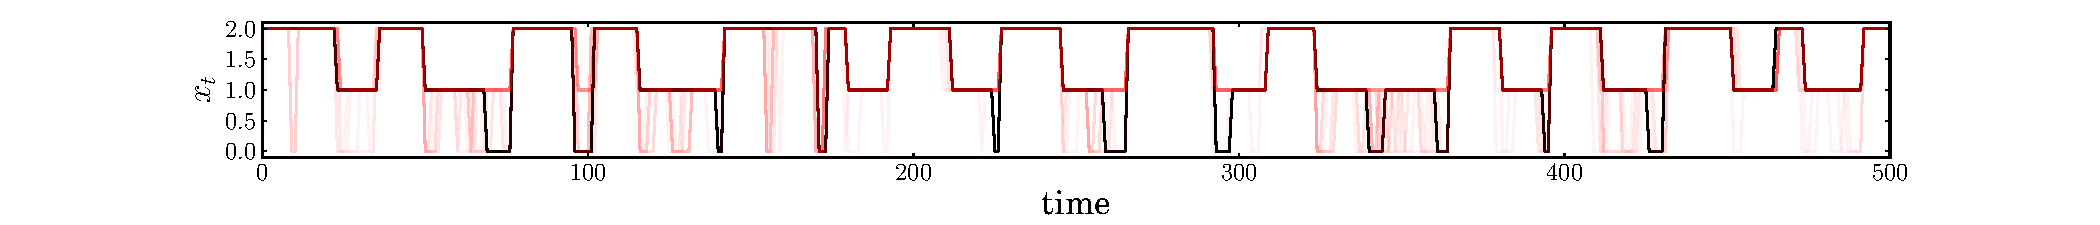
\includegraphics[width=0.5\textwidth]{../pic/experiment_3_X.pdf}
        \label{fig:exp_2_state}
    } \\
    \subfloat[][]{
        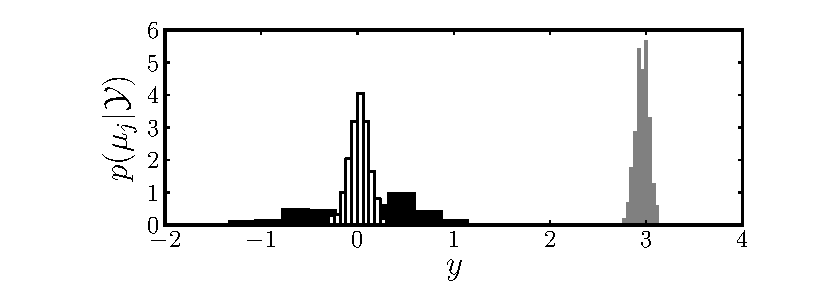
\includegraphics[width=0.25\textwidth]{../pic/posterior_means_exp3.pdf}
        \label{fig:posterior_means_3}
    } 
    \subfloat[][]{
        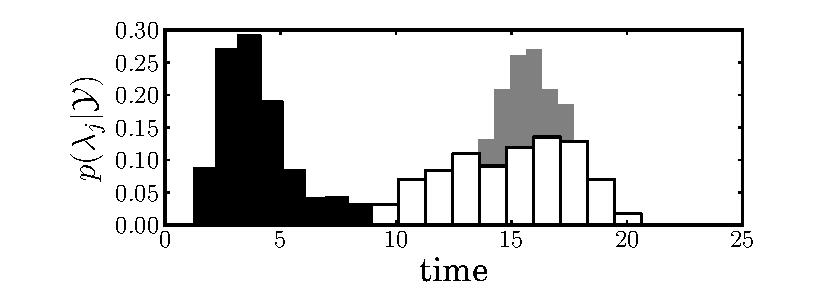
\includegraphics[width=0.25\textwidth]{../pic/posterior_rates_exp3.pdf}
        \label{fig:posterior_rates_3}
    }
    \caption{Beam sampler results from a system with identical observation distributions but differing durations. Observations are shown in a); true states in b) overlaid with 20 state traces produced by the sampler. Here we have parameters $\mu_1 = \mu_2 = 0$, $\mu_3 = 3$ and $\lambda_1 = 5$, $\lambda_2 = 15$, $\lambda_3 = 20$. Samples from the posterior observation-mean and duration-rate distributions are shown in c) and d), respectively.}
    \label{fig:experiment2_results}
\end{figure}
